The scenario damage calculator computes damage distribution statistics for all
\glspl{asset} in a given \gls{exposuremodel} for a single specified
\gls{rupture}. Damage distribution statistics include the mean and standard
deviation of damage fractions for different damage states. This calculator
requires the definition of a finite \gls{rupturemodel}, an \gls{exposuremodel}
and a \gls{fragilitymodel}; the main results are the damage distribution
statistics per \gls{asset}, aggregated damage distribution statistics per
taxonomy, aggregated damage distribution statistics for the region, and
collapse maps, which contain the spatial distribution of the number or area of
collapsed buildings throughout the region of interest.

The \gls{rupture} characteristics---i.e. the magnitude, hypocenter and fault
geometry---are modelled as deterministic in the scenario calculators. Multiple
simulations of different possible \glspl{acr:gmf} due to the single
\gls{rupture} are generated, taking into consideration both the inter-event
variability of ground motions, and the intra-event residuals obtained from a
spatial correlation model for ground motion residuals. The use of logic trees
allows for the consideration of uncertainty in the choice of a ground motion
model for the given tectonic region.

As an alternative to computing the \glspl{acr:gmf} with \glsdesc{acr:oqe},
users can also provide their own sets of \glspl{acr:gmf} as input to the
scenario damage calculator.

\textbf{Note}: The damage simulation algorithm for the scenario damage 
calculator has changed starting from \glsdesc{acr:oqe39} to use a full
Monte Carlo simulation of damage states.

For each \gls{acr:gmf}, a damage state is simulated for each building for every
\gls{asset} in the \gls{exposuremodel} using the provided \gls{fragilitymodel},
and finally the mean damage distribution across all realizations is calculated.
The calculator also provides aggregated damage distribution statistics for the
portfolio, such as mean damage fractions for each taxonomy in the 
\gls{exposuremodel}, and the mean damage for the entire region of study.

The required input files required for running a scenario damage calculation
and the resulting output files are depicted in Figure~\ref{fig:io-structure-scenario-damage}.

\begin{figure}[ht]
\centering
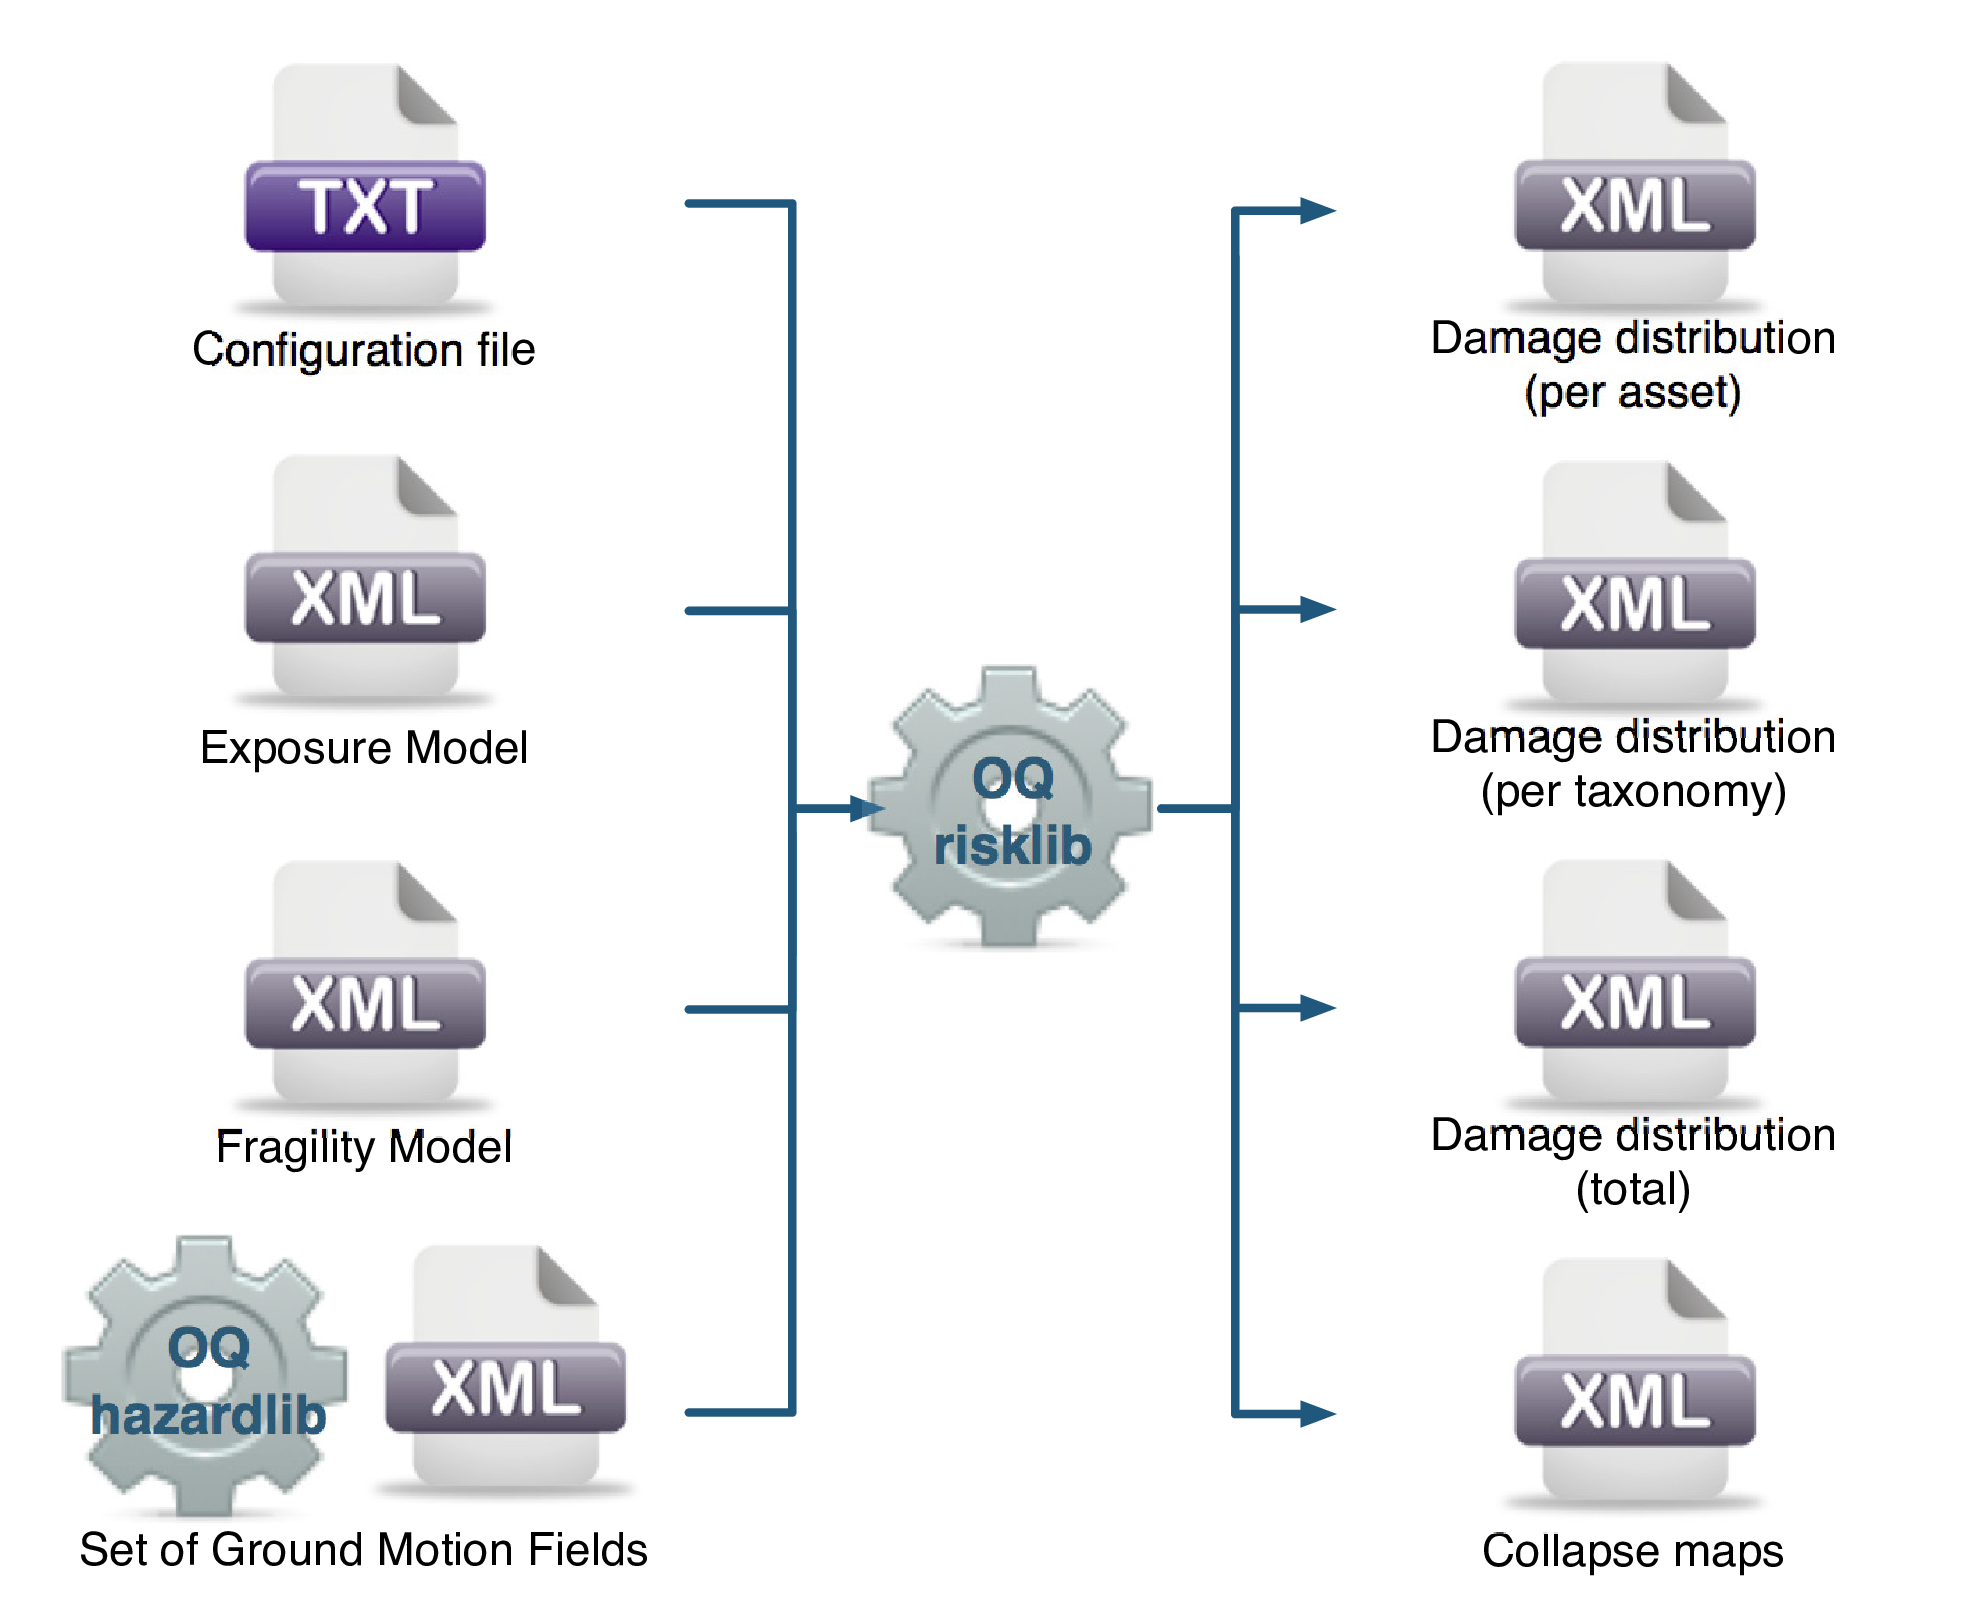
\includegraphics[width=9cm,height=7cm]{figures/risk/io-structure-scenario-damage.pdf}
\caption{Scenario Damage Calculator input/output structure.}
\label{fig:io-structure-scenario-damage}
\end{figure}

\gls{consequencemodel} files can also be
provided as inputs for a scenario damage calculation in addition to
\glspl{fragilitymodel} files, in order to estimate consequences based on the
calculated damage distribution. The user may provide one
\gls{consequencemodel} file corresponding to each loss type (amongst
structural, nonstructural, contents, and business interruption) for which a
\gls{fragilitymodel} file is provided. Whereas providing a
\gls{fragilitymodel} file for at least one loss type is mandatory for running
a Scenario Damage calculation, providing corresponding \gls{consequencemodel}
files is optional.
